% ----- formatovani dokumentu -----------------------------------------------
\documentclass[12pt,a4paper,titlepage,final]{report}
\usepackage[utf8]{inputenc}
\usepackage[T1, IL2]{fontenc}
\usepackage{graphicx}
\usepackage{epstopdf}
\usepackage[margin=2cm]{caption}
\usepackage{subcaption}
\usepackage{float}
\usepackage[top=3cm, left=2cm, right=2cm, text={17cm, 24cm}, ignorefoot]{geometry}
\usepackage{color}
\usepackage{url}
\usepackage{setspace}
\singlespacing
\usepackage[square, numbers]{natbib} 
\pagestyle{plain}
\pagenumbering{arabic}
\setcounter{page}{1}
\setcounter{secnumdepth}{-1}
\setlength{\parindent}{1cm}	
\usepackage{natbib}



% ----- vyberte jazyk -------------------------------------------------------
\usepackage[english,czech]{babel}
%\usepackage[english]{babel}

% ----- dopiste titulky -----------------------------------------------------
\newcommand\Course{Počítačová grafika}
\newcommand\WorkTitle{Procedurální texturování pomocí shaderů}
\newcommand\AuthorA{Zdeněk Biberle}
\newcommand\AuthorAEmail{xbiber00@stud.fit.vutbr.cz}
\newcommand\AuthorB{Tomáš Šujan}
\newcommand\AuthorBEmail{xsujan02@stud.fit.vutbr.cz}
\newcommand\AuthorC{Zdeněk Tretter}
\newcommand\AuthorCEmail{xtrett00@stud.fit.vutbr.cz}
\newcommand\Faculty{Fakulta Informačních Technologií}
\newcommand\School{Vysoké Učení Technické v Brně}

\usepackage[
pdftitle={\WorkTitle},
pdfauthor={\AuthorA, \AuthorB, \AuthorC},
bookmarks=true,
colorlinks=true,
breaklinks=true,
urlcolor=blue,
citecolor=blue,
linkcolor=blue,
unicode=true,
]
{hyperref}


% ----- titulni strana ------------------------------------------------------

\begin{document}
	\begin{titlepage}
	\begin{center}
		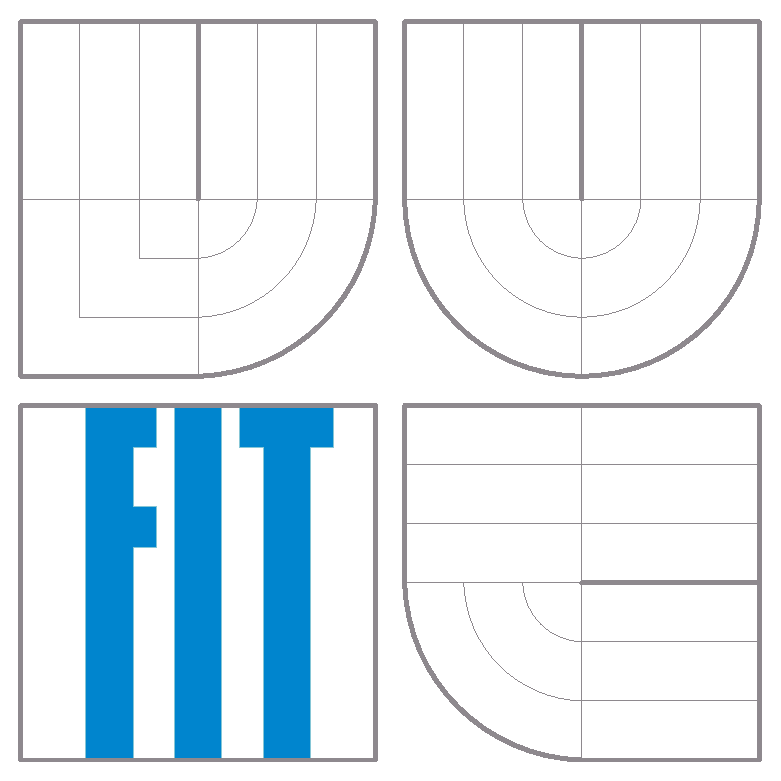
\includegraphics[height=5cm]{images/logo.eps}
	\end{center}
	\vfill
	\begin{center}
		\begin{Large}
			\Course\\
		\end{Large}
		\bigskip
		\begin{Huge}
			\WorkTitle\\
		\end{Huge}
	\end{center}
	\vfill
	\begin{center}
		\begin{large}
			\today
		\end{large}
	\end{center}
	\vfill
	\begin{flushleft}
		\begin{large}
			\begin{tabular}{lll}
				Autoři: & \AuthorA, & \url{\AuthorAEmail} \\
				        & \AuthorB, & \url{\AuthorBEmail} \\
				        & \AuthorC, & \url{\AuthorCEmail} \\
				& & \\
				& \Faculty \\
				& \School \\
			\end{tabular}
		\end{large}
	\end{flushleft}
\end{titlepage}		
	
% ----- obsah --------------------------------------------------------------
	
\tableofcontents

% ----- zadani -------------------------------------------------------------
\newpage
\chapter{Zadání}

\begin{itemize}
	\item Implementace jednoduché platformy pro experimentování s tvorbou procedurálních textur s následujícími vlastnostmi:
	\begin{itemize}
		\item Zobrazení různých modelů.
		\item Poskytnutí funkcí vhodných pro generování procedurálních textur
		\item Odezva na změny v shaderech v reálném čase nebo alespoň na požádání (každopádně bez nutnosti restartovat či dokonce překompilovávat aplikaci).
		\item Možnost vizualizace nejen obrazových dat pro snažší nalezení problémů.
	\end{itemize}
	\item Prozkoumání a případná implementace generování nejen barevných dat, kupříkladu:
	\begin{itemize}
		\item Data pro techniky jako bump mapping, normal mapping, parallax mapping.
		\item koeficienty odrazivosti světla a jiné vlastnosti materiálů týkající se světla.
	\end{itemize}
	\item Implementace různě vypadajících a různě složitých textur využitím dostupných vlastností hlavní aplikace.
	\item Prozkoumání a případná implementace animovaných textur.
\end{itemize}

%---------------------------------------------------------------------------
\chapter{Nejdůležitější dosažené výsledky}

\section{Normálové mapy}

Naše aplikace umožňuje, aby jednotlivé texturovací shadery generovaly nejenom barevnou složku textury, ale i její normálovou mapu. To může v praxi být poměrně náročná operace, která vyžaduje nemalé množství maticových či vektorových operací, ovšem její vizuální přínos je značný. Příkladem budiž textura drevo.glsl, jejíž barevná složka, kterou vidíme na obrázku~\ref{fig:drevo-color}, není příliš zajímavá, ovšem přidáním normálové mapy dle obrázku~\ref{fig:drevo-normal} dostaneme mnohem zajímavější výsledek, viditelný na obrázku~\ref{fig:drevo-full}.

\begin{figure}[h]
	\centering
	\begin{subfigure}[b]{0.40\textwidth}
		\captionsetup{type=figure}
		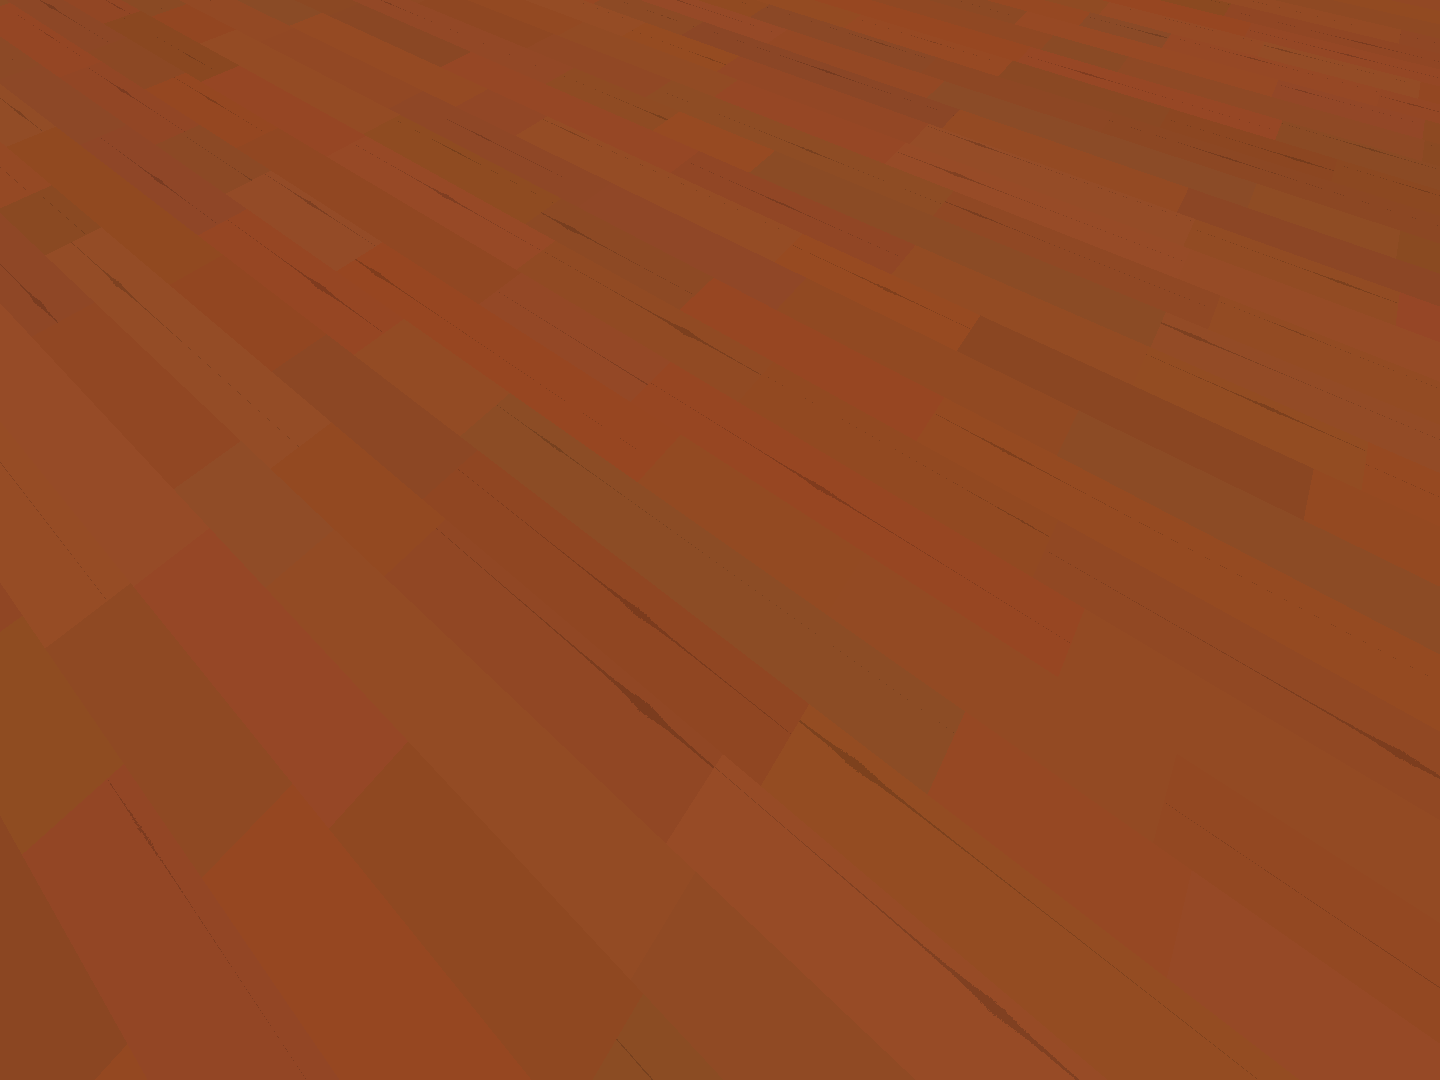
\includegraphics[width=\textwidth]{images/drevo-color.png}
		\captionof{figure}{Barevná složka textury drevo.glsl}
		\label{fig:drevo-color}
	\end{subfigure}
	\begin{subfigure}[b]{0.40\textwidth}
		\captionsetup{type=figure}
		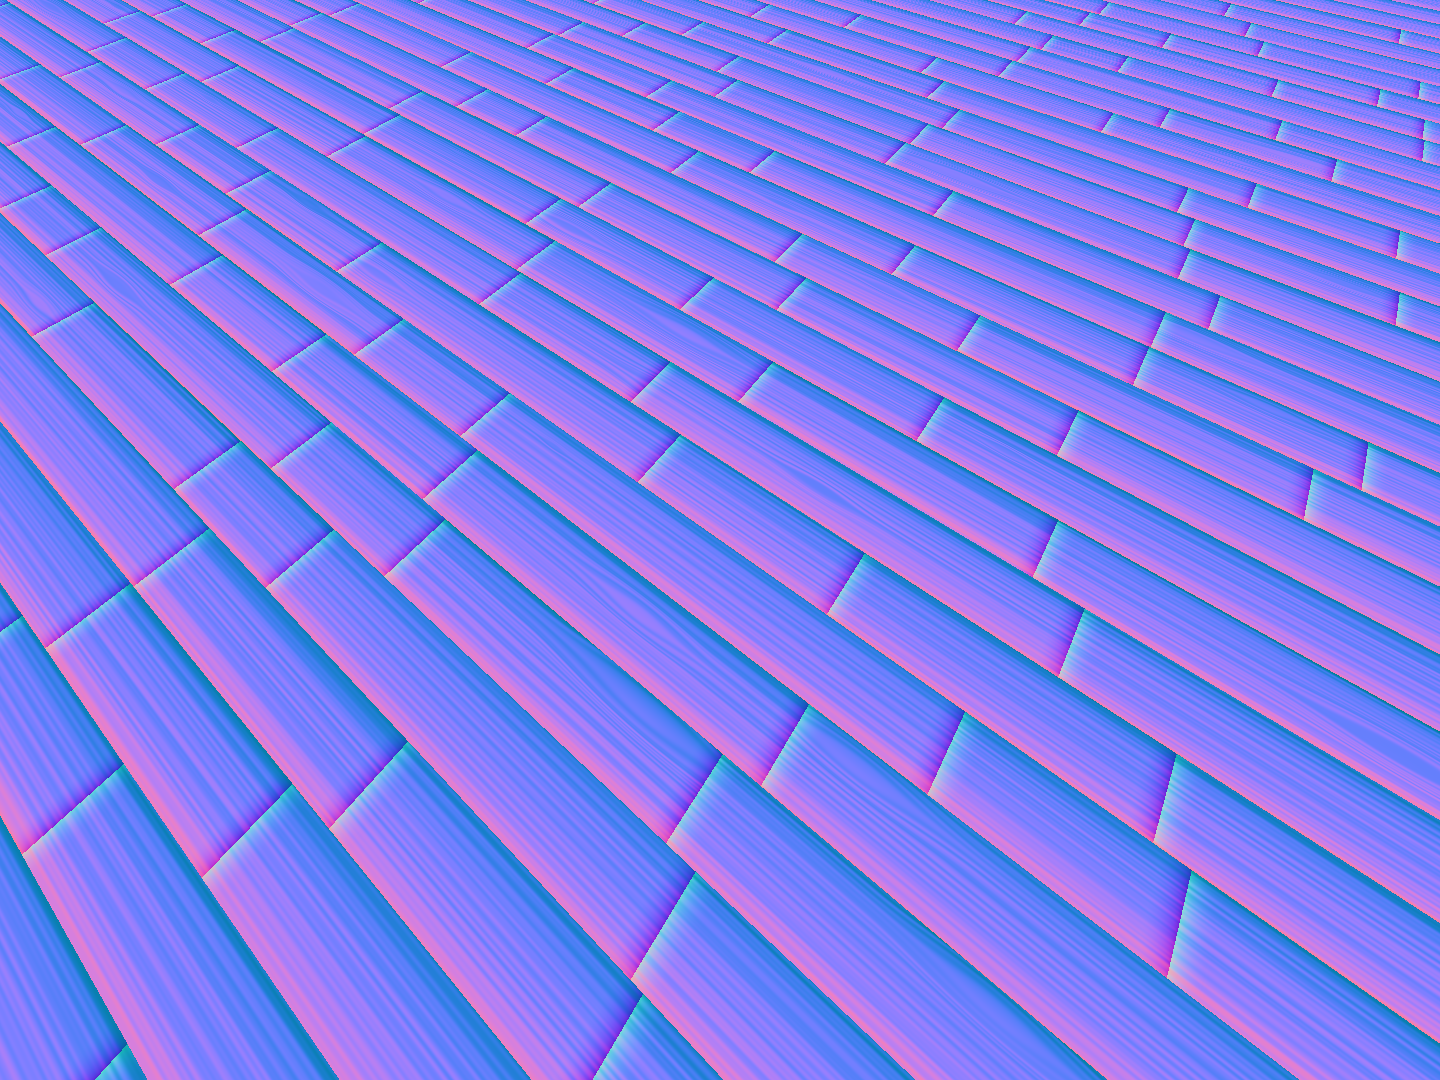
\includegraphics[width=\textwidth]{images/drevo-normal.png}
		\captionof{figure}{Normálová mapa textury drevo.glsl}
		\label{fig:drevo-normal}
	\end{subfigure}
	
	\begin{subfigure}[b]{0.60\textwidth}
		\captionsetup{type=figure}
		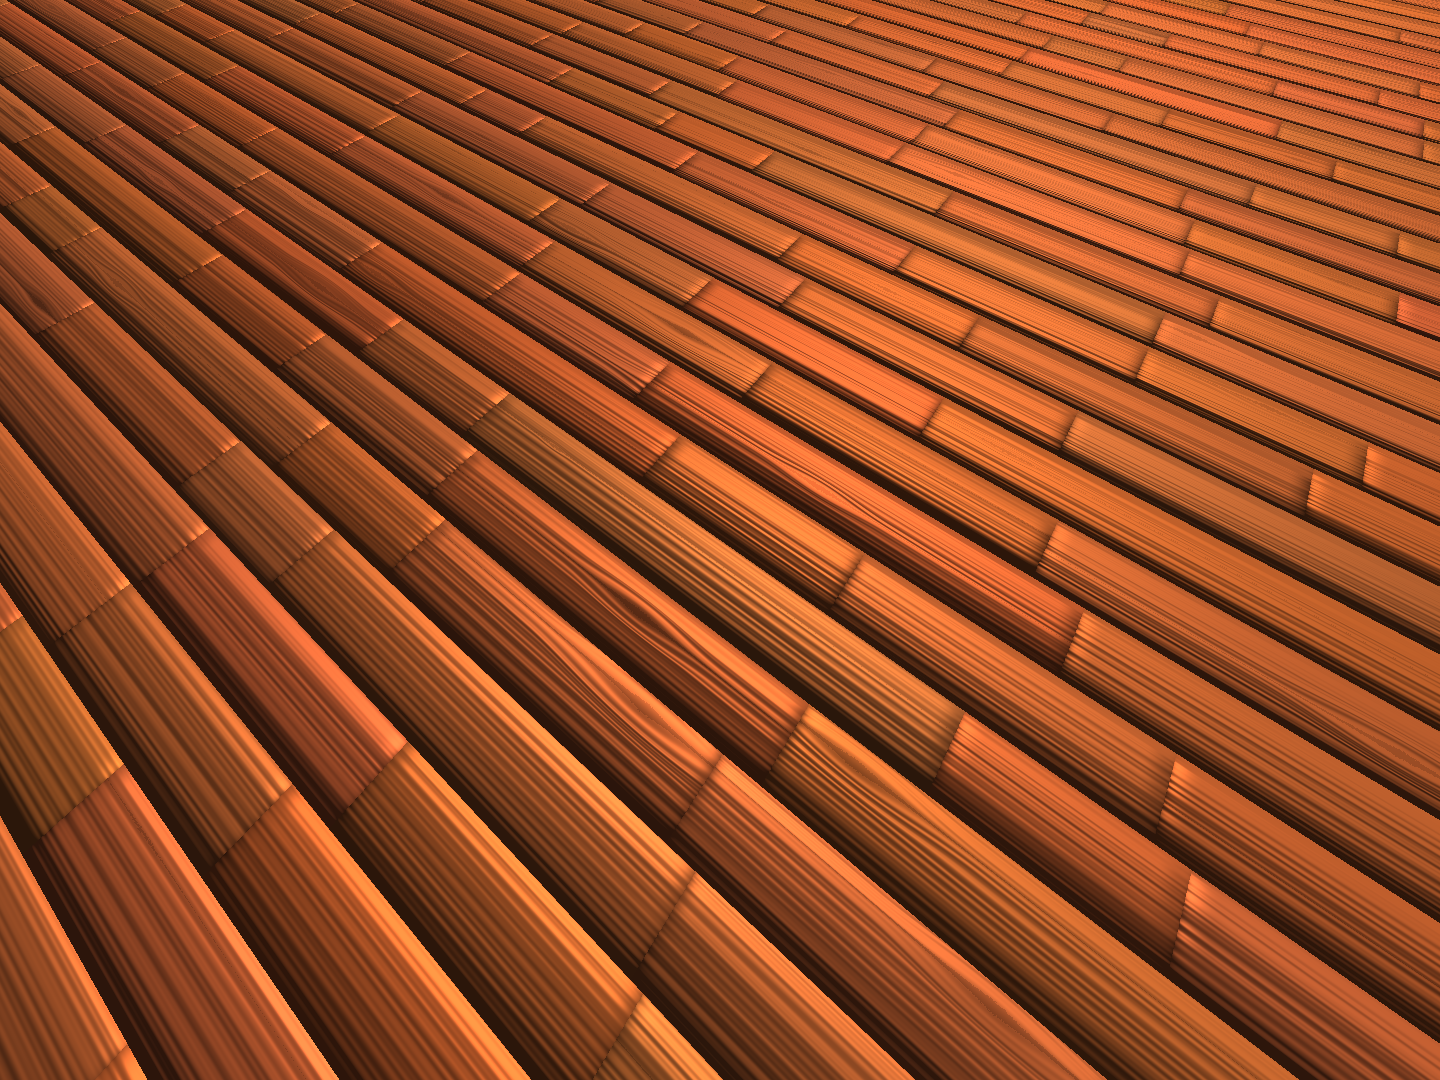
\includegraphics[width=\textwidth]{images/drevo-full.png}
		\captionof{figure}{Finální vzhled textury drevo.glsl}
		\label{fig:drevo-full}
	\end{subfigure}
\end{figure}

\section{Textura dlazba.glsl}

\begin{figure}[h]
	\centering
	\captionsetup{type=figure}
	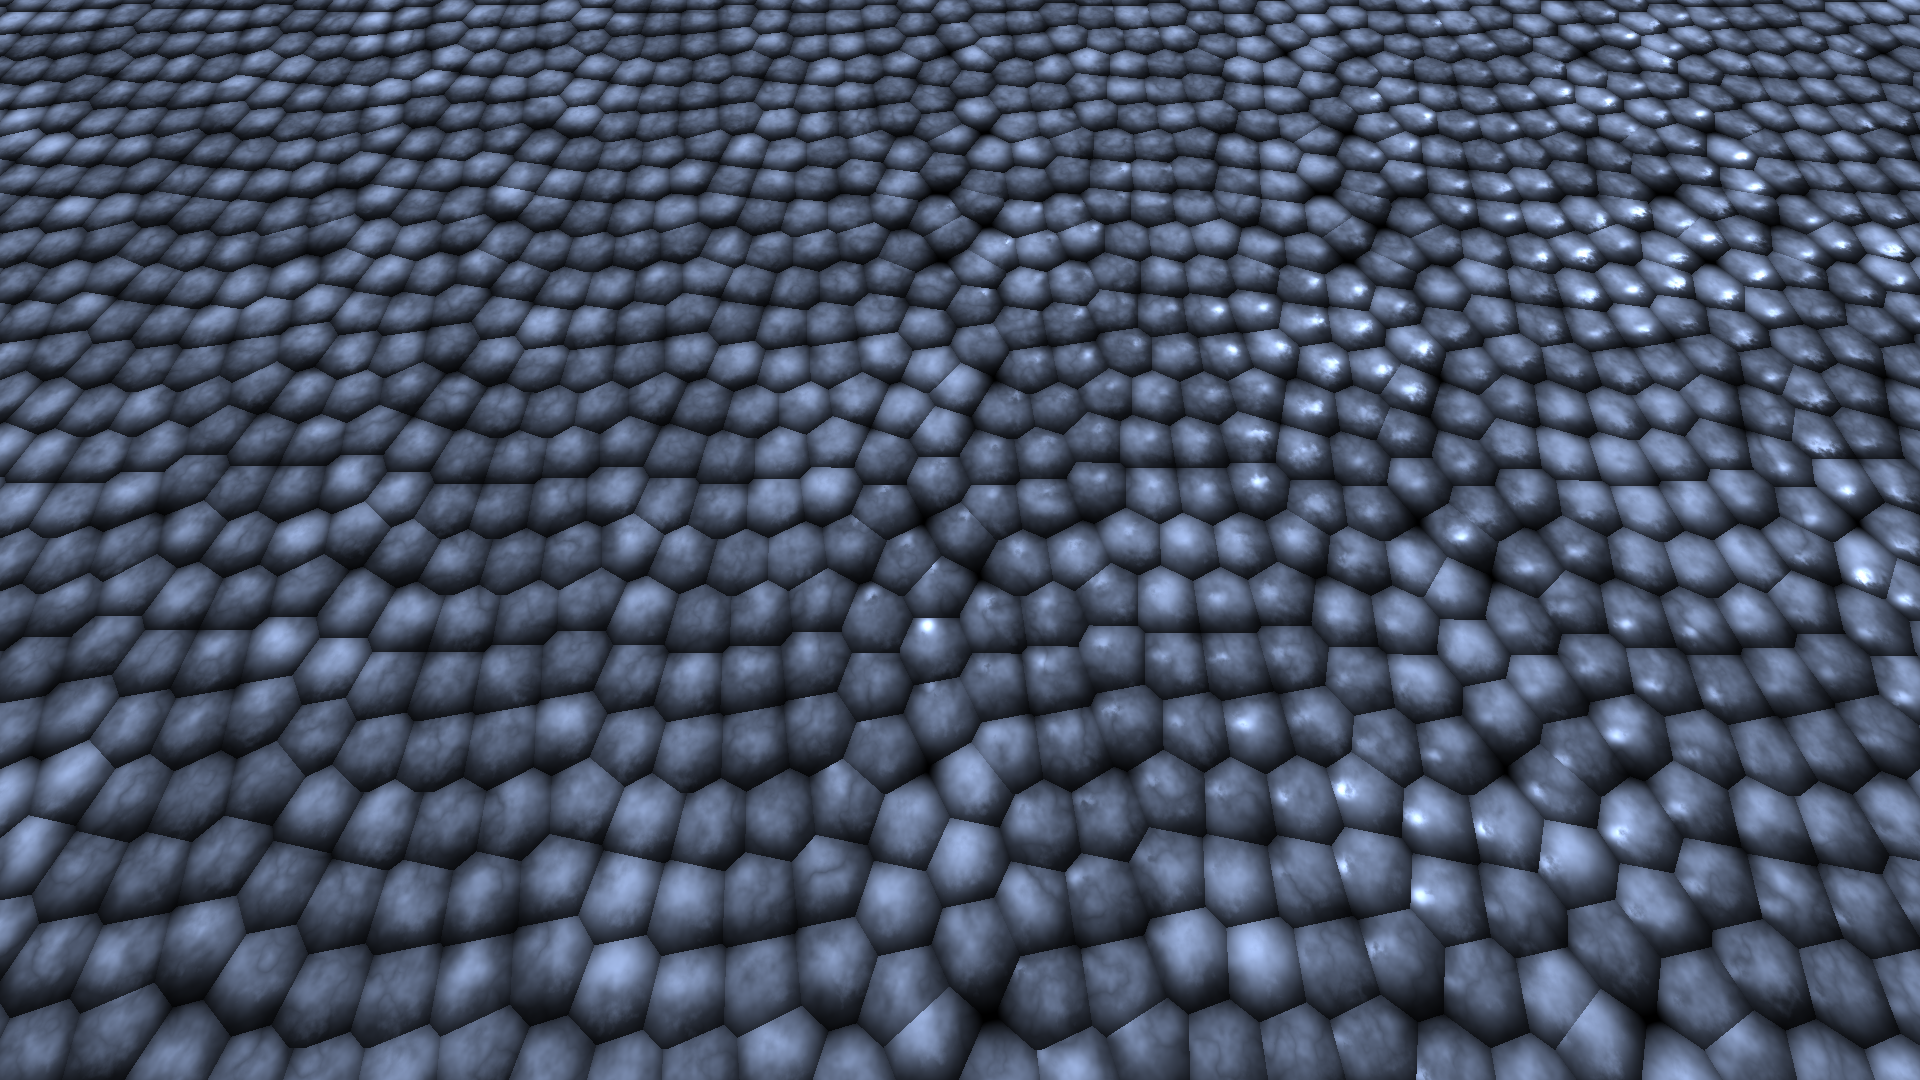
\includegraphics[width=\textwidth]{images/dlazba.png}
	\captionof{figure}{Textura dlazba.glsl}
\end{figure} 

Pôvodne mali byť moje textúry dve - mramorový povrch a bunková štruktúra. Mramorová dlažba mala byť pokrytá šumom, ktorý som získal prenásobením jemného šumu (snoise) so sínusovým vzorom, na ktorý bola potom aplikovaná turbulencia. Do tejto kombinácie bola nakoniec vnásobená farba mramoru. Výsledok bol ale veľmi nekvalitný. Nový návrh - bunkový vzor - vytvorený spojením viacerých šumových a permutačných funkcií dle \cite{gustavson2014} vyzeral celkom prijateľne po pridaní bledomodrej farby, no zároveň tiež veľmi fádne a plasticky. Ako riešenie som zvolil spojenie oboch textúr do jednej - bunky som upravil tak, aby pripomínali dlažbový vzor, a na ne som aplikoval mramorový šum. Navyše som do výpočtu zahrnul výpočet normály pre jednotlivé bunky - dlažobné kocky, čo má za následok pseudo-priestorový vzhľad. Na spekulárne osvetlenie som tiež aplikoval tento šum, čo má za následok fakt, že dlažba sa neleskne všade rovnako, ale "novšie" kocky (teda tie s menším pokrytím mramorového šumu) sa lesknú viac, ako tie "obchodené" - viac zašumené. Výstupom je relatívne kvalitná textúra, ktorá by sa dala použiť v skutočnom projekte.

\section{Textura mraky.glsl}
\begin{figure}[h]
	\captionsetup{type=figure}
	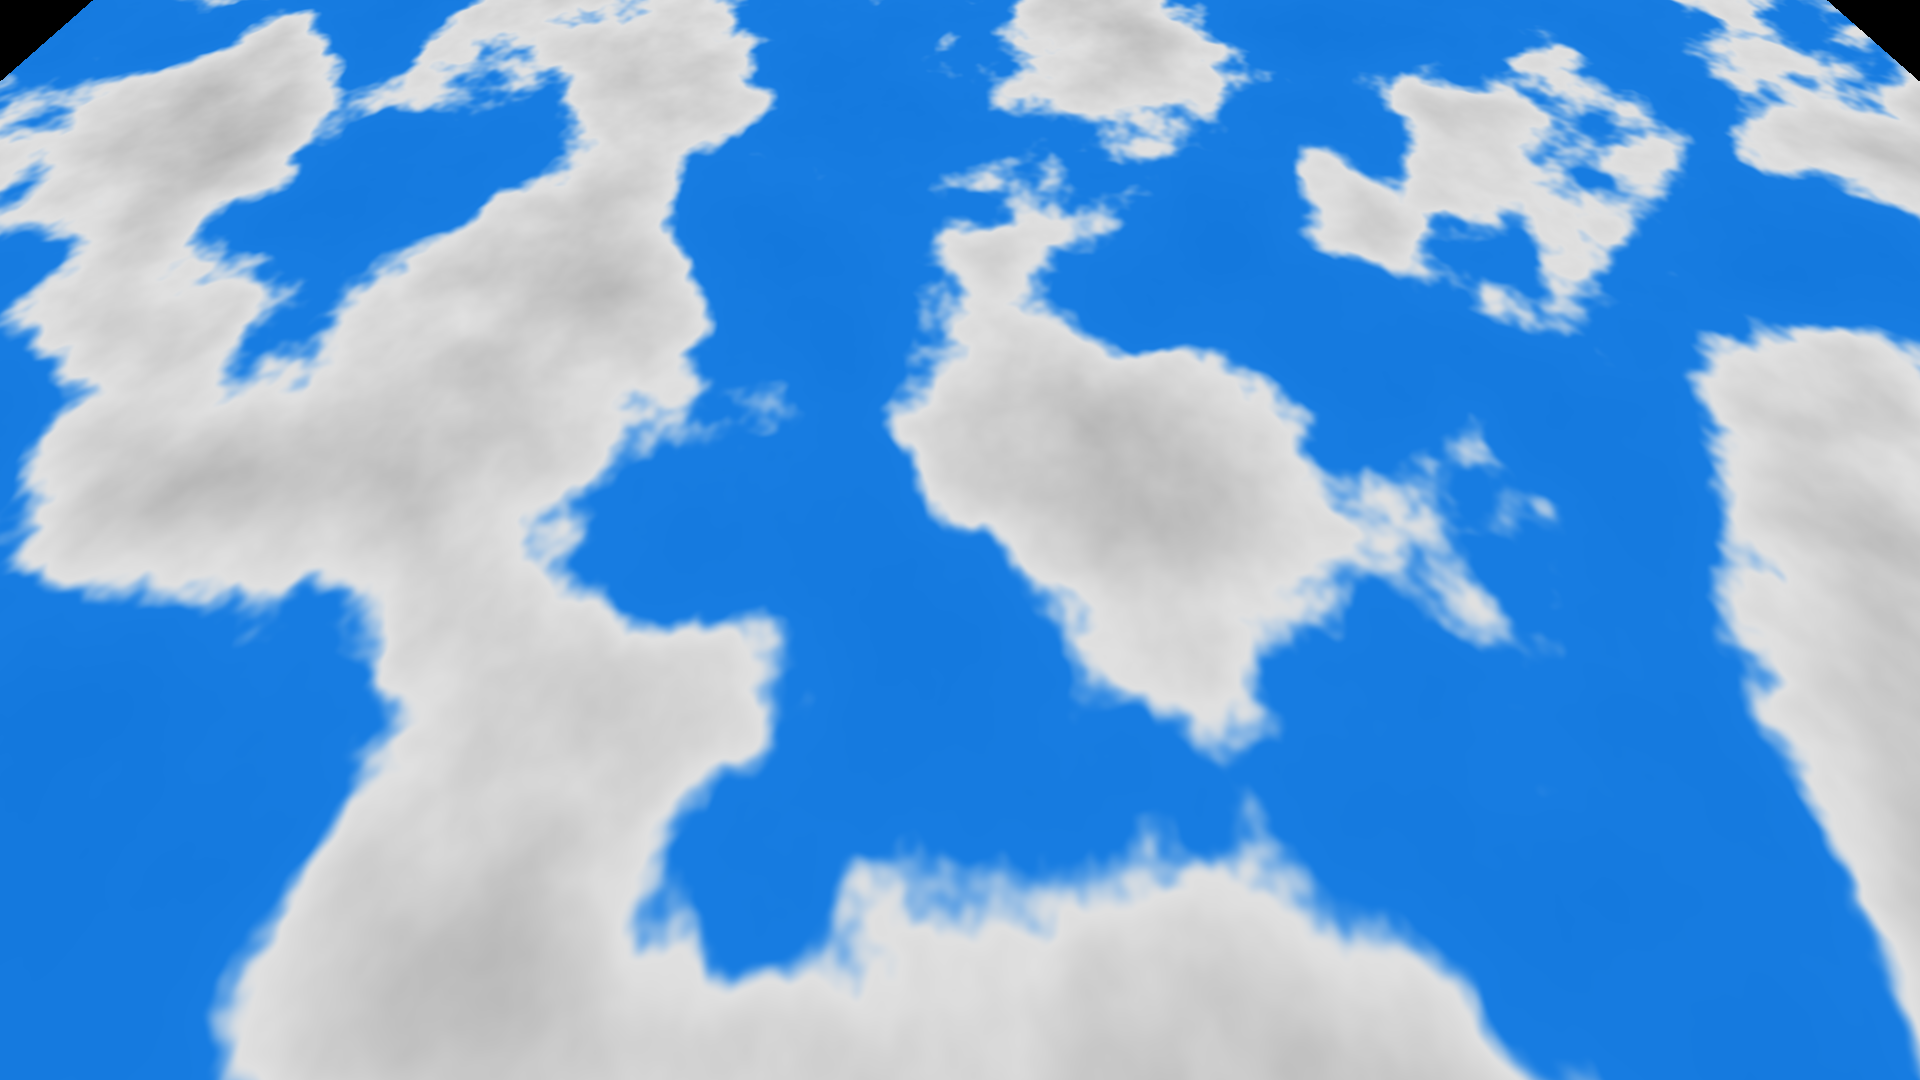
\includegraphics[width=\textwidth]{images/mraky.png}
	\captionof{figure}{Textura mraky.glsl}
\end{figure}

Jednoduchá a přesto slušně uvěřitelná textura mraků, které se navíc pohybují a mění. 

Právě změna tvaru mraků je  na této textuře zajímavá. Tvar mraků je generovaný pomocí turbulence doplněné o posun závislý na čase v jedné ze složek.
  


%---------------------------------------------------------------------------
\chapter{Zvláštní použité znalosti}
Pro generování alespoň trochu realistických textur je nutné mít k dispozici nějaký zdroj šumu, ideálně více než jeden druh. Ačkoliv se generování a vlastnostem šumu a náhodných jevů věnovalo na FIT hned několik předmětů, tak využití znalostí v těchto předmětech získaných bylo v tomto projektu poměrně obtížné. 

Architektura grafických karet a vykreslovacího řetězce například dělá použití jednoduchých kongruentních generátorů šumu v praxi nemožné. Stejně tak je nereálné použití různých frekvenčních filtrů na šumových datech a získání různě frekvenčně omezených šumových signálů.

Informace, které by byly užitečné pro tento projekt, přinesla až přednáška z předmětu Počítačová grafika, která se ale uskutečnila až příliš pozdě. Je ale pochopitelné, že z časových důvodů musí k něčemu takovému dojít.

%---------------------------------------------------------------------------
\chapter{Práce na projektu}

\begin{itemize}
\item \textbf{\AuthorA}: Aplikace, zpracování a UV mapování modelů, obecné shadery, textury drevo.glsl, kamuflaz.glsl a digitalnikamuflaz.glsl
\item \textbf{\AuthorB}: Textura dlazba.glsl
\item \textbf{\AuthorC}: Textury kachlicky.glsl, jeansy.glsl, mraky.glsl a mrakyNaHladine.glsl
\end{itemize}

%---------------------------------------------------------------------------
\section{Co bylo nejpracnější}

\begin{itemize}
\item \textbf{\AuthorA}: Jelikož doplnění textur o normálové mapy byl původně můj nápad, tak také bylo na mě, abych tuto techniku implementoval. Až později jsem ovšem zjistil, že pro mapování normál nestačí znát pouze normálové vektory jednotlivých vrcholů modelu, ale je nutné mít k dispozici celý tangentní prostor. Poté jsem začal experimentovat s výpočtem tangentního prostoru pomocí knihovny Open Asset Import Library i mého vlastního řešení. Nakonec kombinací obou metod dorazil k řešení, které stále není ideální, ale obecně funguje poměrně obstojně.
\item \textbf{\AuthorB}: Najpracnejšou časťou projektu bola z môjho pohľadu konsolidácia návrhu textúry do samotného fragment shaderu. Svoje teoretické nápady na procedurálnu generáciu textúr som musel niekoľkokrát pozmeniť. Výsledkom môjho prvotného návrhu bola nekvalitná textúra.  Algoritmus výpočtu šumu som pozmenil a vytvoril som novú textúru znázorňujúcu bunkovú štruktúru, no oba výsledky boli tentoraz fádne a jednoliate. Nakoniec som tieto dva návrhy zlúčil do jedného. Výsledná textúra má relatívne komplexný vzhľad aj za použitia normál, ktorý by dve textúry samy o sebe určite nedosiahli. Jednu dobu sa na kockách objavovali grafické artefakty, ktoré boli spôsobené nekorektným otočením normálovéhu uhlu - na nesprávnu stranu. Pracné bolo teda vymyslieť také riešenie, aby moja dovtedajšia práca nebola stratená, ale zároveň, aby výsledkom bola relatívne kvalitná textúra, ktorá bude mať aj určitú priestorovú komplexnosť.
\item \textbf{\AuthorC}: Největším problémem u mě bylo projekt přeložit, abych mohl začít pracovat. Na OS Windows se mi nedařilo správně nainstalovat všechny potřebné knihovny a vše správně nastavit. Linux zase nechtěl spolupracovat s mojí AMD grafickou kartou. A integrovaná grafická karta nepodporovala vyšší verze OpenGL. Nakonec jsem programoval přes VNC u Zdeňka Biberleho. 

Co se týče samotného programování, tak nebylo jednoduché odhadnout, jak se jednotlivé OpenGL funkce zachovají na různé vstupy. O to složitější to bylo při jejich kombinaci, proto jsem měl vždy na začátku jen základní představu, jak by měla výsledná textura vypadat. Postupně jsem pak vymýšlel detaily, jejichž implementace si ale mnohdy vyžádala i značné změny již napsaného kódu, což bylo časově náročné. 

\end{itemize}


%---------------------------------------------------------------------------
\section{Zkušenosti získané řešením projektu}

\begin{itemize}
\item \textbf{\AuthorA}: Prohloubení znalostí o geometry shaderech, tangentních prosterech, normal mappingu a příjemné zjištění, že SDL2 je mnohem schopnější, než SDL1.2.
\item \textbf{\AuthorB}:
\item \textbf{\AuthorC}: Seznámení s jazykem GLSL, programování v něm, poznání čeho je schopen a práce přes VNC.
\end{itemize}

%---------------------------------------------------------------------------
\chapter{Autoevaluace}

\paragraph{Technický návrh (80\%):} Celý projekt je poměrně vhodně rozdělen na jednoduché podproblémy a zpravidla se jedná o platformu vhodnou pro experimentování s generováním různě složitých procedurálních textur.

\paragraph{Programování (80\%):} Z tohoto pohledu je aplikace kvalitně zpracovaná, ovšem místy je slabě komentovaná. To je zjevné primárně u zdrojových kódů samotných textur, které jsou plné zdánlivě náhodně použitých funkcí a magických konstant.

\paragraph{Vzhled vytvořeného řešení (75\%):} Estetická kvalita je přijatelná, ale rozhodně ne dokonalá. Bylo by možné ji vylepšit například lepším mapováním textur na zvolené modely.

\paragraph{Využití zdrojů (60\%):} Bylo využito několik zdrojů týkajících se primárně generování šumu, a to jak kód, tak i teoretické základy. Zbytek aplikace byl vytvořen použitím intuice a představivosti. Obecně mohlo být zdrojů použito více.

\paragraph{Hospodaření s časem (50-90\%, jak kdo):} Práce na projektu začala dokonce i dříve, než byl projekt oficiálně zaregistrován. I přesto byly činnosti přiřazené některým členům týmu dokončeny později, než bylo očekáváno. Navzdory tomu je projekt dokončen a nemá žádné výrazné nedostatky.

\paragraph{Spolupráce v týmu (50\%):} Ukázalo se, že tlačit Zdeňka Trettera a Tomáše Šujana do práce silněji by bylo rozumné. Jinak ale vše proběhlo bez problémů.

\paragraph{Celkový dojem (80\%):} Díky kreativní povaze tohoto projektu se jednalo o příjemnou novou zkušenost. Jelikož byly vlastnosti finálního produktu stanoveny velice volně, tak byl každý člen týmu omezen pouze svou představivostí. 

Výsledná aplikace je dostatečně jednoduchá a zároveň dostatečně schopná na to, aby i člověk v oblasti generování procedurálních textur nezkušený byl schopný vyprodukovat nějaké výsledky.

%---------------------------------------------------------------------------
\chapter{Ovládání vytvořeného programu}

\section{Technologie potřebné pro spuštění programu}
\paragraph{Softwarové púožadavky}
\begin{itemize}
	\item Knihovna SDL2 - Vytvoření a ovládání okna aplikace a OpenGL kontextu.
	\item Knihovna GLEW - Nahrávání OpenGL funkcí.
	\item Knihovna Open Asset Import Library - Nahrávání modelů.
\end{itemize}

\paragraph{Hardwarové požadavky}
\begin{itemize}
	\item Grafická karta s podporou alespoň OpenGL 3.3.
\end{itemize}

\section{Programy a služby použité při tvorbě}
\begin{itemize}
	\item Blender - Úprava a tvorba modelů a mapování textur.
\end{itemize}

\section{Obsluha programu}
\begin{itemize}
	\item Pohyb
		\begin{itemize}
			\item Levétlačítko myši - Držením tohoto tlačítka a pohybem myši lze rotovat se zobrazeným modelem.
			\item Kolečko myši - Přiblížení a oddálení modelu.
		\end{itemize}
	\item Zobrazení
		\begin{itemize}

			\item Klávesa R - Zapíná a vypíná autonomní rotaci modelu.
			\item Klávesa T - Zapíná a vypíná zobrazení tangentního prostoru modelu.
			\item Klávesa A - Zapíná plné zobrazení textury, tj. včetně normálového mapování a osvětlení.
			\item Klávesa S - Zapíná zobrazení pouze barevné složky textury.		\item Klávesa D - Zapíná zobrazení pouze normálové složky textury.
			\item Klávesa F - Zapíná zobrazení pouze osvětlení.
		\end{itemize}
	\item Ostatní
		\begin{itemize}
			\item Klávesa F5 - Opětovné nahrání a zkompilování shaderů.
			\item Šipky doleva a doprava - Přepíná mezi texturovacími shadery.
		\end{itemize}
\end{itemize}

Soubor se zobrazovaným modelem je programu předán jako první parametr, ostatní parametry pak specifikují texturovací shadery, mezi kterými lze přepínat.

%---------------------------------------------------------------------------
\chapter{Doporučení pro budoucí zadávání projektů}

Témata projektů byla zadána dostatečně brzy a byl tak dostatek času pro zvolení toho správného. Taktéž termín odevzdání byl stanoven rozumně. 

Zadání nebyla příliš striktní, což je určitě pozitivní.

%---------------------------------------------------------------------------

%\chapter{Různé}

%Ještě něco by v dokumentaci mělo být? Napište to sem! Podle potřeby i založte novou kapitolu.

%---------------------------------------------------------------------------

\bibliographystyle{plain}
\nocite{gustavson2014,mcewan2012,lengyel}
\bibliography{reference}
\addcontentsline{toc}{chapter}{Literatura}

\end{document}

